% Indicate the main file. Must go at the beginning of the file.
% !TEX root = ../main.tex

%%%%%%%%%%%%%%%%%%%%%%%%%%%%%%%%%%%%%%%%%%%%%%%%%%%%%%%%%%%%%%%%%%%%%%%%%%%%%%%%
% 04_discussion
%%%%%%%%%%%%%%%%%%%%%%%%%%%%%%%%%%%%%%%%%%%%%%%%%%%%%%%%%%%%%%%%%%%%%%%%%%%%%%%%


\section{Discussion}
\label{discussion}

\subsection{Hyperparameter Tuning}%%%%%%%%%%%%%%%%%%%%%%%%%%%%%%%%%%%%%%%%%%%%%%



\subsection{Performance of the best Model}%%%%%%%%%%%%%%%%%%%%%%%%%%%%%%%%%%%%%%

Using the best performing configuration it is worth to take a closer look to the
training process of the model. The validation accuracy and loss at the end of
every epoch is shown in \autoref{fig:loss_acc_best}. The graphs show a typical
training process. The validation accuracy is increasing while the validation loss
is decreasing. Towards the end both graphs are flattening out which is a sign that
the model was not learning anymore when the training was stopped. So the patience
of 100 for the early stopping was an appropriate choice. Since the validation loss
and accuracy are very noisy it was necessary to use a patience that high. This might
be a sign, that the data processing or the model architecture could be improved.

%==== figure: loss_acc_best ====%
\begin{figure}[h]
\centering
\captionsetup{width=0.9\linewidth}
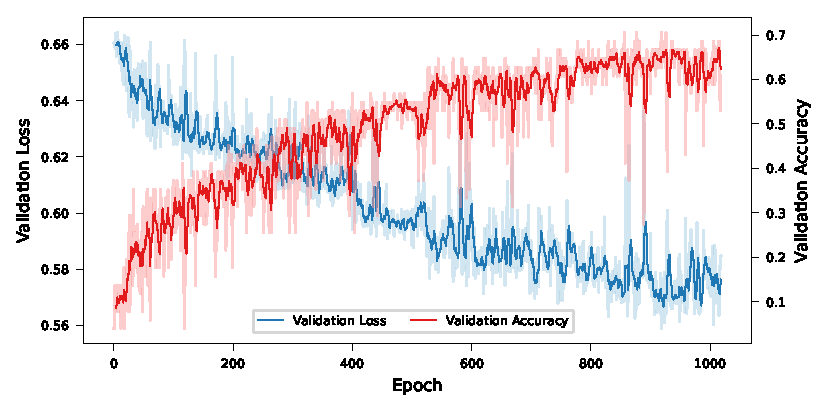
\includegraphics[width=1.0\textwidth]{figures/loss_acc_best.pdf}
\caption{The validation loss and accuracy of the best model. Light version is not smoothed and dark version is smoothed with a window size of 5.}
\label{tab:loss_acc_best}
\end{figure}

%===============================%

In the original paper \autocite{faissAdaptiveRepresentationsSound2023}
the model was used on different datasets and with different models. Furthermore the model was
run five times with different seeds and the accuracy was averaged. The model using a MelSpectrogram
frontend on the InsectSet32 dataset achieved an mean accuracy of 0.6 with a range of 0.57 to 0.65
on the validation set and an accuracy of 0.62 with a range of 0.57 to 0.67 on the test set.
The best performing configuration for the model in this study achieves an accuracy of 0.706 on the validation set
and an accuracy of 0.649. For the test set this is well in the range of the original paper.
Why the model in this study performs better on the validation set compared to the difference
between the validation and test set in the original paper is not clear. The accuracy achieved
by the model with the other frontend from the original paper is unreached by the model in this study.
So there is still room for improvement.


